%\section{Introduction}

\section{Motivation of the research}
Today, a great number of people in the world can not spend a day without using smartphones or personal computers(PCs) to retrieve information from the Internet for work or for daily life.
For example, people use these devices to look up web pages, emails, social media and sometimes to play games.
These services are often called web applications, where information is delivered using Hyper Text Transfer Protocols(HTTP) or Hypertext Transfer Protocol Secure (HTTPS) from servers at the other end of the Internet.
Web applications are provided by various organizations, including commercial companies, government, non-profitable organizations, schools, etc.
A client program on PCs or smartphone sends out requests to servers and the servers respond with data that is requested, using HTTP or HTTPS. 

Servers for web applications are usually computers located in a data center.
%Servers also refer to the server programs that are runing on these computers. 
Multiple servers cooperate to fulfill the need of the clients.
A group of these servers is often called a web application cluster or a web cluster.
Figure~\ref{fig:web_cluster} shows schematic diagram of an example of a web cluster.

\begin{figure}[h]
\begin{center}
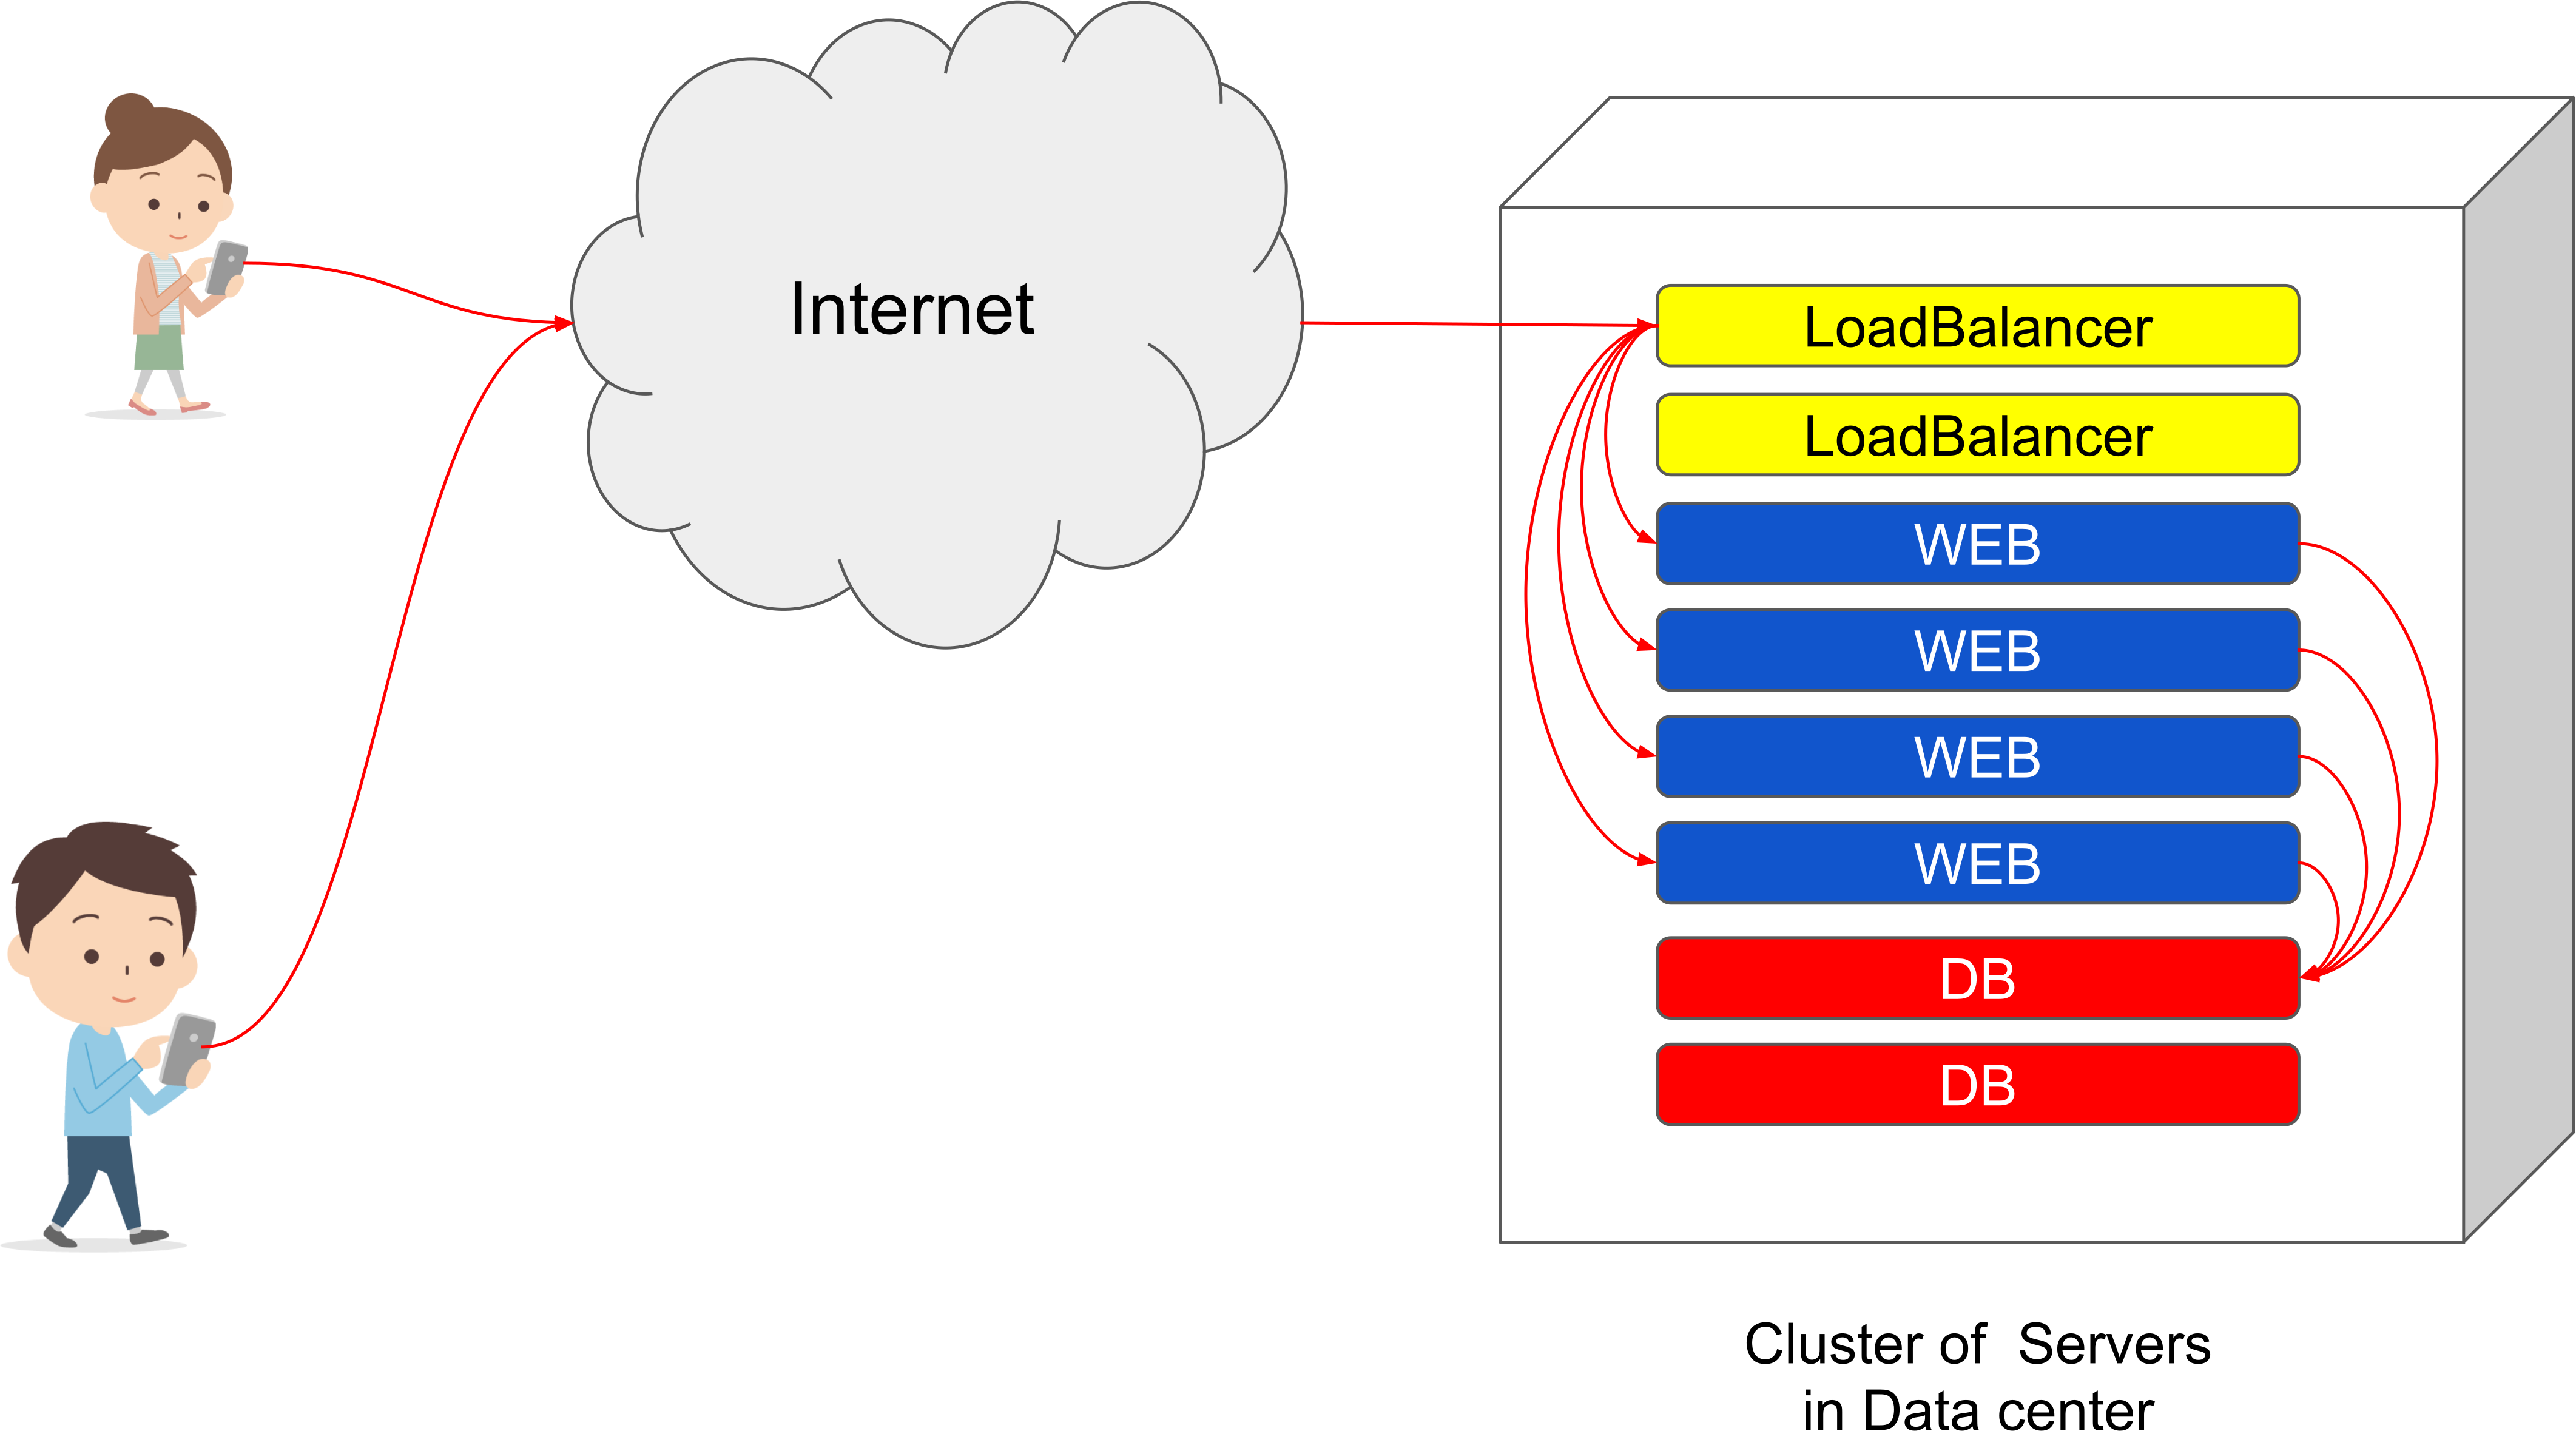
\includegraphics[width=0.8\columnwidth]{Figs/web_cluster.png}
\end{center}
\caption{
An example of web cluster.
}
\label{fig:web_cluster}
\end{figure}

In this example, there are two load balancers, four web servers and two Database(DB) servers that work together to respond to requests from clients.
The load balancers distribute requests from clients to multiple web servers. 
Then the web servers retrieve some data from the database servers to form the response, sometimes they may store important data into the database servers.
Web application providers often purchase these servers and locate them in server housing facilities called data centers.

The emergence of Cloud Computing made it easier for web application providers to deploy their services than before.
Cloud providers offer to lend virtual machines(VM), which share a single physical server.
Web application providers needed to buy or rent physical servers and install them in a data center before they start their services.
But now, thanks to Cloud Computing, they can rent VMs in pay-as-you-go bases with the matter of several clicks in their office, and they are charged with finer granularities.
For cloud users (i.e., web application providers), Cloud Computing lowers initial cost spent on infrastructures for their services and also gives them agility, i.e., shortens the time to prepare servers in a data center for their service.
And at the time when the computing resources for a service is excessive, users can quickly decrease the VMs and reduce the cost.
This was impossible when they bought servers and installed them in the datacenter.

More recently, Linux containers\cite{menage2007adding} have come to draw a significant amount of attention because they are lightweight, portable, and reproducible, and hence cloud providers are starting to offer services utilizing container technologies.
Linux containers are generally more lightweight than virtual machines(VMs), because the containers share the kernel with the host operating system (OS), while they maintain separate execution environments.
Linux containers can be run on top of widely used Linux OS; therefore they can be run in most of the cloud infrastructures and on-premise data centers.
They are generally portable because the process execution environments are archived into tar files,
so whenever one attempts to run a container, the exact same file systems are restored from the archives even when totally different data centers are used.
This means that containers can provide reproducible and portable execution environments.

For the same reasons, Linux containers are attractive for web applications as well, and it is expected that web applications consisting of a cluster of containers are capable of being migrated easily for a variety of purposes.
For example disaster recovery, cost performance optimizations, meeting legal compliance and shortening the geographical distance to customers are the main concerns for web application providers in e-commerce, gaming, Financial technology(Fintech) and Internet of Things(IoT) field.

The purpose of this research is to enable web application providers to easily deploy their services across the world seamlessly, regardless of cloud providers or data centers they use, by better-utilizing container cluster technology. 
Also, the author aims to realize the future where users can choose whatever infrastructure they like without sacrificing advanced features that are provided only by limited cloud providers.

\section{Avoid lock-in problem}

It is desirable if users can migrate their services to multiple of cloud providers or on-premise data centers seamlessly, which spread across the world.
Container cluster management systems facilitate these usages by functioning as middlewares, which hide the differences among cloud providers and on-premise data centers.

Kubernetes\cite{K8s2017}, which is one of the most popular container cluster management systems, enables easy deployment of container clusters.
Kubernetes are initially developed by engineers inside Google, to facilitate container cluster deployment for web applications.
Kubernetes allows users to deploy a cluster of containers each of which depends on each other, with the ease of launching a single application program.
It also allows users to increase or decrease the number of containers dynamically depending on the amount of traffic that they have to respond.

Since Kubernetes is expected to hide the differences in the base environments, it is expected that users can easily deploy a web application on different cloud providers or on on-premise data centers, without adjusting the container cluster configurations to the new environment. 
This allows a user to easily migrate a web application consisting of a container cluster even to the other side of the world.
A typical web application migration scenario is; 
a user starts the container cluster in the new location, route the traffic there, then stop the old container cluster at his or her convenience.

However, this scenario only works when the user migrates a container cluster among major cloud providers including Google Cloud Platform (GCP), Amazon Web Applications (AWS), and Microsoft Azure.
This is because Kubernetes fails to completely hide differences in base environments.
Kubernetes does not provide generic ways to route the traffic from the internet into container cluster running in the Kubernetes and expects the base infrastructure automatically route traffic to nodes that might host container.
In other words, Kubernetes is heavily dependent on cloud load balancers, which is external load balancers that are set up on the fly by cloud providers through their application protocol interfaces (APIs).
Once the traffic reaches the nodes, Kubernetes handles it nicely, but this is a problem since not every cloud provider or on-premise data center has load balancers that can be set up through API and utilized by Kubernetes.
Other container cluster management systems, e.g. Docker swarm, etc, also lack a generic way to route the traffic into the container cluster.
Therefore this is one of the generic problems that current container cluster architectures possess.

Load balancers are often used to distribute high volume traffic from the Internet to thousands of web servers.
They are implemented as dedicated hardware or software on commodity hardware.
Major cloud providers have developed software load balancers\cite{eisenbud2016maglev,patel2013ananta} as a part of their infrastructures.
They claim that their load balancers have a high-performance level and scalability.
Those software load balancers have APIs through which an outside program can set up and control the behavior of the load balancers.
Once cloud load balancers are set up automatically and distribute incoming traffic to every server that hosts containers,
the traffic is then distributed again to destination containers using the iptables destination network address translation(DNAT)\cite{MartinA.Brown2017,Marmol2015} rules in a round-robin manner.

In the case of on-premise data centers, there are variety of proprietary hardware load balancers.
It is very likely that most of the load balancers are left unsupported by Kubernetes, even if some of the load balancers may have APIs through which a container management system can set up and control the behavior.
In these cases, the user needs to manually configure the static route for inbound traffic in an ad-hoc manner.
Since the Kubernetes fails to provide a uniform environment from a container cluster viewpoint, migrating container clusters among the different environments will always require daunting tasks.
One of the aims of this study is to seek a generic way to route the traffic into container clusters automatically, by providing a software load balancer that works well with the container management systems, and thereby to facilitate web application migrations.

\section{Contribution}

In order to achieve these aims, the author proposes a portable and scalable software load balancer that can be used in any environment including cloud providers and in on-premise data centers.
By using such a load balancer, users do not need to manually adjust their services to the base infrastructures.
As a proof of concept the author implements the proposed software load balancer that works well with with Kubernetes using following technologies;
1) To make the load balancer usable in any environment, Linux kernel's Internet Protocol Virtual Server (ipvs)\cite{Zhang2000} is containerized using Docker\cite{merkel2014docker}. 
2) To make the load balancer redundant and scalable, the author makes it capable of updating the routing table of upstream router with Equal Cost Multi-Path(ECMP) routes\cite{al2008scalable} using a standard protocol, Border Gateway Protocol(BGP).
3) The author also extends the research into implementing the novel load balancer using eXpress Data Plane(XDP) technology\cite{bertin2017xdp} to enhance the performance level to meet the need for 10Gbps network speed.

Contributions of this paper are as follows:
Although there have been studies regarding redundant software load balancers especially from the major cloud providers\cite{eisenbud2016maglev,patel2013ananta}, their load balancers are only usable within their respective cloud infrastructures.
Therefore in order to facilitate container cluster migrations, a software load balancer architecture with redundancy and scalability that is common to any base infrastructure has been needed.
This paper aims to provide such a load balancer architecture and evaluate a proof-of-concept system that is built using Open Source Software(OSS) technologies.
The understanding obtained from a detailed analysis of the evaluation also helps both the research community and the web application industry, because there does not exist enough of them.
Moreover, since proposed load balancer architecture uses nothing but existing OSSs and standard Linux boxes, users can build a cluster of redundant load balancers in their environment.

The outcome of this study will benefit users who want to deploy their web applications on any cloud provider where no scalable load balancer is provided, to achieve high scalability.
Moreover, the result of our study will potentially benefit users who want to use a group of different cloud providers and on-premise data centers across the globe seamlessly.
In other words, users will become being able to deploy a complex web application on aggregated computing resources on the earth, as if they were starting a single process on a single computer.

\section{Outline}

The rest of the paper is organized as follows.
Chapter \ref{chapter:background} provides the background information and related works.
Chapter \ref{chapter:architecture} provides the problems of existing load balancers and proposes suitable architectures.
Chapter \ref{chapter:implemetation} presents implementation of the proposed load balancer architecture in detail.
Chapter \ref{chapter:portablelb} discusses portability and performance levels of the proposed load balancer in 1 Gbps network environment.
Chapter \ref{chapter:redundancy} discusses the redundancy and scalability of the proposed load balancers.
Chapter \ref{chapter:performance} present the performance levels of the proposed load balancer in 10 Gbps network environment and discuss the method to improve the performance of a software load balancer.
Chapter \ref{chapter:futurework} discusses the limitation and the future work of this study,
which is followed by a conclusion of this work in Chapter \ref{Conclusions}.





